% Created by tikzDevice version 0.12.6 on 2024-03-03 13:25:00
% !TEX encoding = UTF-8 Unicode
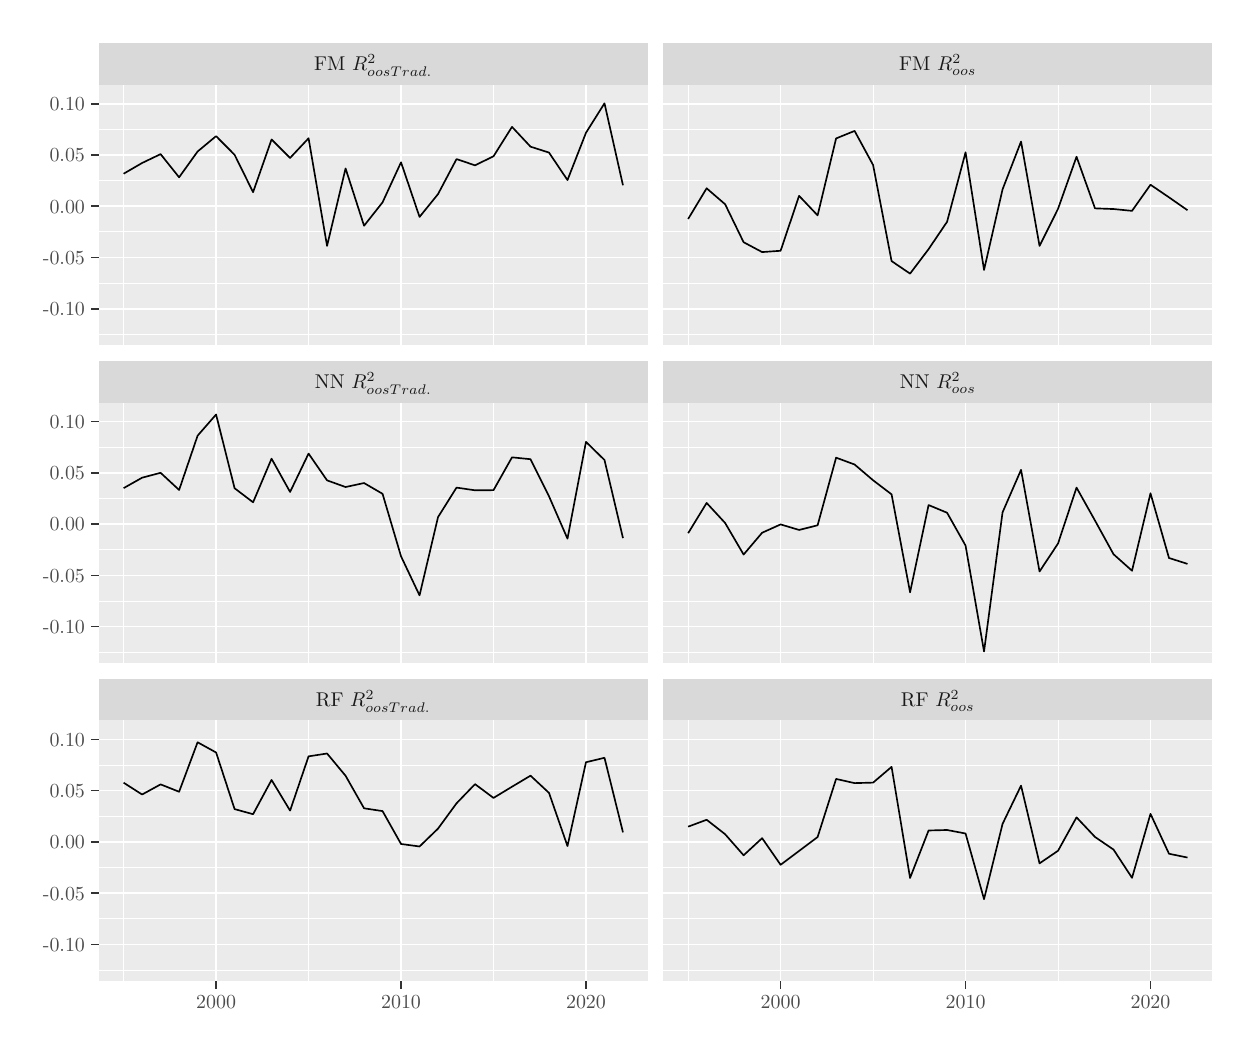
\begin{tikzpicture}[x=1pt,y=1pt]
\definecolor{fillColor}{RGB}{255,255,255}
\path[use as bounding box,fill=fillColor,fill opacity=0.00] (0,0) rectangle (433.62,361.35);
\begin{scope}
\path[clip] (  0.00,  0.00) rectangle (433.62,361.35);
\definecolor{drawColor}{RGB}{255,255,255}
\definecolor{fillColor}{RGB}{255,255,255}

\path[draw=drawColor,line width= 0.6pt,line join=round,line cap=round,fill=fillColor] (  0.00,  0.00) rectangle (433.62,361.35);
\end{scope}
\begin{scope}
\path[clip] ( 25.65,246.50) rectangle (224.13,340.69);
\definecolor{fillColor}{gray}{0.92}

\path[fill=fillColor] ( 25.65,246.50) rectangle (224.13,340.69);
\definecolor{drawColor}{RGB}{255,255,255}

\path[draw=drawColor,line width= 0.3pt,line join=round] ( 25.65,250.51) --
	(224.13,250.51);

\path[draw=drawColor,line width= 0.3pt,line join=round] ( 25.65,269.03) --
	(224.13,269.03);

\path[draw=drawColor,line width= 0.3pt,line join=round] ( 25.65,287.55) --
	(224.13,287.55);

\path[draw=drawColor,line width= 0.3pt,line join=round] ( 25.65,306.08) --
	(224.13,306.08);

\path[draw=drawColor,line width= 0.3pt,line join=round] ( 25.65,324.60) --
	(224.13,324.60);

\path[draw=drawColor,line width= 0.3pt,line join=round] ( 34.67,246.50) --
	( 34.67,340.69);

\path[draw=drawColor,line width= 0.3pt,line join=round] (101.50,246.50) --
	(101.50,340.69);

\path[draw=drawColor,line width= 0.3pt,line join=round] (168.33,246.50) --
	(168.33,340.69);

\path[draw=drawColor,line width= 0.6pt,line join=round] ( 25.65,259.77) --
	(224.13,259.77);

\path[draw=drawColor,line width= 0.6pt,line join=round] ( 25.65,278.29) --
	(224.13,278.29);

\path[draw=drawColor,line width= 0.6pt,line join=round] ( 25.65,296.81) --
	(224.13,296.81);

\path[draw=drawColor,line width= 0.6pt,line join=round] ( 25.65,315.34) --
	(224.13,315.34);

\path[draw=drawColor,line width= 0.6pt,line join=round] ( 25.65,333.86) --
	(224.13,333.86);

\path[draw=drawColor,line width= 0.6pt,line join=round] ( 68.08,246.50) --
	( 68.08,340.69);

\path[draw=drawColor,line width= 0.6pt,line join=round] (134.91,246.50) --
	(134.91,340.69);

\path[draw=drawColor,line width= 0.6pt,line join=round] (201.74,246.50) --
	(201.74,340.69);
\definecolor{drawColor}{RGB}{0,0,0}

\path[draw=drawColor,line width= 0.6pt,line join=round] ( 34.67,308.57) --
	( 41.35,312.45) --
	( 48.03,315.65) --
	( 54.72,307.28) --
	( 61.40,316.60) --
	( 68.08,322.15) --
	( 74.77,315.41) --
	( 81.45,301.90) --
	( 88.13,320.95) --
	( 94.82,314.28) --
	(101.50,321.38) --
	(108.18,282.49) --
	(114.87,310.48) --
	(121.55,289.77) --
	(128.23,298.22) --
	(134.91,312.70) --
	(141.60,292.96) --
	(148.28,301.21) --
	(154.96,313.85) --
	(161.65,311.61) --
	(168.33,314.87) --
	(175.01,325.50) --
	(181.70,318.35) --
	(188.38,316.21) --
	(195.06,306.28) --
	(201.74,323.36) --
	(208.43,334.01) --
	(215.11,304.39);
\end{scope}
\begin{scope}
\path[clip] ( 25.65,131.66) rectangle (224.13,225.84);
\definecolor{fillColor}{gray}{0.92}

\path[fill=fillColor] ( 25.65,131.66) rectangle (224.13,225.84);
\definecolor{drawColor}{RGB}{255,255,255}

\path[draw=drawColor,line width= 0.3pt,line join=round] ( 25.65,135.66) --
	(224.13,135.66);

\path[draw=drawColor,line width= 0.3pt,line join=round] ( 25.65,154.18) --
	(224.13,154.18);

\path[draw=drawColor,line width= 0.3pt,line join=round] ( 25.65,172.71) --
	(224.13,172.71);

\path[draw=drawColor,line width= 0.3pt,line join=round] ( 25.65,191.23) --
	(224.13,191.23);

\path[draw=drawColor,line width= 0.3pt,line join=round] ( 25.65,209.75) --
	(224.13,209.75);

\path[draw=drawColor,line width= 0.3pt,line join=round] ( 34.67,131.66) --
	( 34.67,225.84);

\path[draw=drawColor,line width= 0.3pt,line join=round] (101.50,131.66) --
	(101.50,225.84);

\path[draw=drawColor,line width= 0.3pt,line join=round] (168.33,131.66) --
	(168.33,225.84);

\path[draw=drawColor,line width= 0.6pt,line join=round] ( 25.65,144.92) --
	(224.13,144.92);

\path[draw=drawColor,line width= 0.6pt,line join=round] ( 25.65,163.44) --
	(224.13,163.44);

\path[draw=drawColor,line width= 0.6pt,line join=round] ( 25.65,181.97) --
	(224.13,181.97);

\path[draw=drawColor,line width= 0.6pt,line join=round] ( 25.65,200.49) --
	(224.13,200.49);

\path[draw=drawColor,line width= 0.6pt,line join=round] ( 25.65,219.01) --
	(224.13,219.01);

\path[draw=drawColor,line width= 0.6pt,line join=round] ( 68.08,131.66) --
	( 68.08,225.84);

\path[draw=drawColor,line width= 0.6pt,line join=round] (134.91,131.66) --
	(134.91,225.84);

\path[draw=drawColor,line width= 0.6pt,line join=round] (201.74,131.66) --
	(201.74,225.84);
\definecolor{drawColor}{RGB}{0,0,0}

\path[draw=drawColor,line width= 0.6pt,line join=round] ( 34.67,194.96) --
	( 41.35,198.73) --
	( 48.03,200.50) --
	( 54.72,194.30) --
	( 61.40,213.91) --
	( 68.08,221.56) --
	( 74.77,194.92) --
	( 81.45,189.84) --
	( 88.13,205.60) --
	( 94.82,193.57) --
	(101.50,207.44) --
	(108.18,197.77) --
	(114.87,195.36) --
	(121.55,196.80) --
	(128.23,192.91) --
	(134.91,170.32) --
	(141.60,156.21) --
	(148.28,184.49) --
	(154.96,195.15) --
	(161.65,194.18) --
	(168.33,194.23) --
	(175.01,206.09) --
	(181.70,205.41) --
	(188.38,192.01) --
	(195.06,176.70) --
	(201.74,211.68) --
	(208.43,205.12) --
	(215.11,176.91);
\end{scope}
\begin{scope}
\path[clip] ( 25.65, 16.81) rectangle (224.13,111.00);
\definecolor{fillColor}{gray}{0.92}

\path[fill=fillColor] ( 25.65, 16.81) rectangle (224.13,111.00);
\definecolor{drawColor}{RGB}{255,255,255}

\path[draw=drawColor,line width= 0.3pt,line join=round] ( 25.65, 20.81) --
	(224.13, 20.81);

\path[draw=drawColor,line width= 0.3pt,line join=round] ( 25.65, 39.34) --
	(224.13, 39.34);

\path[draw=drawColor,line width= 0.3pt,line join=round] ( 25.65, 57.86) --
	(224.13, 57.86);

\path[draw=drawColor,line width= 0.3pt,line join=round] ( 25.65, 76.38) --
	(224.13, 76.38);

\path[draw=drawColor,line width= 0.3pt,line join=round] ( 25.65, 94.90) --
	(224.13, 94.90);

\path[draw=drawColor,line width= 0.3pt,line join=round] ( 34.67, 16.81) --
	( 34.67,111.00);

\path[draw=drawColor,line width= 0.3pt,line join=round] (101.50, 16.81) --
	(101.50,111.00);

\path[draw=drawColor,line width= 0.3pt,line join=round] (168.33, 16.81) --
	(168.33,111.00);

\path[draw=drawColor,line width= 0.6pt,line join=round] ( 25.65, 30.07) --
	(224.13, 30.07);

\path[draw=drawColor,line width= 0.6pt,line join=round] ( 25.65, 48.60) --
	(224.13, 48.60);

\path[draw=drawColor,line width= 0.6pt,line join=round] ( 25.65, 67.12) --
	(224.13, 67.12);

\path[draw=drawColor,line width= 0.6pt,line join=round] ( 25.65, 85.64) --
	(224.13, 85.64);

\path[draw=drawColor,line width= 0.6pt,line join=round] ( 25.65,104.17) --
	(224.13,104.17);

\path[draw=drawColor,line width= 0.6pt,line join=round] ( 68.08, 16.81) --
	( 68.08,111.00);

\path[draw=drawColor,line width= 0.6pt,line join=round] (134.91, 16.81) --
	(134.91,111.00);

\path[draw=drawColor,line width= 0.6pt,line join=round] (201.74, 16.81) --
	(201.74,111.00);
\definecolor{drawColor}{RGB}{0,0,0}

\path[draw=drawColor,line width= 0.6pt,line join=round] ( 34.67, 88.52) --
	( 41.35, 84.25) --
	( 48.03, 87.91) --
	( 54.72, 85.25) --
	( 61.40,103.13) --
	( 68.08, 99.44) --
	( 74.77, 78.98) --
	( 81.45, 77.14) --
	( 88.13, 89.51) --
	( 94.82, 78.43) --
	(101.50, 98.04) --
	(108.18, 99.07) --
	(114.87, 91.03) --
	(121.55, 79.27) --
	(128.23, 78.26) --
	(134.91, 66.38) --
	(141.60, 65.47) --
	(148.28, 71.93) --
	(154.96, 81.06) --
	(161.65, 88.00) --
	(168.33, 83.02) --
	(175.01, 87.07) --
	(181.70, 91.06) --
	(188.38, 84.84) --
	(195.06, 65.62) --
	(201.74, 95.91) --
	(208.43, 97.52) --
	(215.11, 70.58);
\end{scope}
\begin{scope}
\path[clip] (229.63,246.50) rectangle (428.12,340.69);
\definecolor{fillColor}{gray}{0.92}

\path[fill=fillColor] (229.63,246.50) rectangle (428.12,340.69);
\definecolor{drawColor}{RGB}{255,255,255}

\path[draw=drawColor,line width= 0.3pt,line join=round] (229.63,250.51) --
	(428.12,250.51);

\path[draw=drawColor,line width= 0.3pt,line join=round] (229.63,269.03) --
	(428.12,269.03);

\path[draw=drawColor,line width= 0.3pt,line join=round] (229.63,287.55) --
	(428.12,287.55);

\path[draw=drawColor,line width= 0.3pt,line join=round] (229.63,306.08) --
	(428.12,306.08);

\path[draw=drawColor,line width= 0.3pt,line join=round] (229.63,324.60) --
	(428.12,324.60);

\path[draw=drawColor,line width= 0.3pt,line join=round] (238.66,246.50) --
	(238.66,340.69);

\path[draw=drawColor,line width= 0.3pt,line join=round] (305.49,246.50) --
	(305.49,340.69);

\path[draw=drawColor,line width= 0.3pt,line join=round] (372.32,246.50) --
	(372.32,340.69);

\path[draw=drawColor,line width= 0.6pt,line join=round] (229.63,259.77) --
	(428.12,259.77);

\path[draw=drawColor,line width= 0.6pt,line join=round] (229.63,278.29) --
	(428.12,278.29);

\path[draw=drawColor,line width= 0.6pt,line join=round] (229.63,296.81) --
	(428.12,296.81);

\path[draw=drawColor,line width= 0.6pt,line join=round] (229.63,315.34) --
	(428.12,315.34);

\path[draw=drawColor,line width= 0.6pt,line join=round] (229.63,333.86) --
	(428.12,333.86);

\path[draw=drawColor,line width= 0.6pt,line join=round] (272.07,246.50) --
	(272.07,340.69);

\path[draw=drawColor,line width= 0.6pt,line join=round] (338.90,246.50) --
	(338.90,340.69);

\path[draw=drawColor,line width= 0.6pt,line join=round] (405.73,246.50) --
	(405.73,340.69);
\definecolor{drawColor}{RGB}{0,0,0}

\path[draw=drawColor,line width= 0.6pt,line join=round] (238.66,292.23) --
	(245.34,303.30) --
	(252.02,297.54) --
	(258.70,283.82) --
	(265.39,280.26) --
	(272.07,280.73) --
	(278.75,300.58) --
	(285.44,293.52) --
	(292.12,321.32) --
	(298.80,324.04) --
	(305.49,311.72) --
	(312.17,277.00) --
	(318.85,272.47) --
	(325.54,281.32) --
	(332.22,291.20) --
	(338.90,316.31) --
	(345.58,273.81) --
	(352.27,302.92) --
	(358.95,320.20) --
	(365.63,282.48) --
	(372.32,295.90) --
	(379.00,314.71) --
	(385.68,296.05) --
	(392.37,295.81) --
	(399.05,295.15) --
	(405.73,304.59) --
	(412.41,300.04) --
	(419.10,295.38);
\end{scope}
\begin{scope}
\path[clip] (229.63,131.66) rectangle (428.12,225.84);
\definecolor{fillColor}{gray}{0.92}

\path[fill=fillColor] (229.63,131.66) rectangle (428.12,225.84);
\definecolor{drawColor}{RGB}{255,255,255}

\path[draw=drawColor,line width= 0.3pt,line join=round] (229.63,135.66) --
	(428.12,135.66);

\path[draw=drawColor,line width= 0.3pt,line join=round] (229.63,154.18) --
	(428.12,154.18);

\path[draw=drawColor,line width= 0.3pt,line join=round] (229.63,172.71) --
	(428.12,172.71);

\path[draw=drawColor,line width= 0.3pt,line join=round] (229.63,191.23) --
	(428.12,191.23);

\path[draw=drawColor,line width= 0.3pt,line join=round] (229.63,209.75) --
	(428.12,209.75);

\path[draw=drawColor,line width= 0.3pt,line join=round] (238.66,131.66) --
	(238.66,225.84);

\path[draw=drawColor,line width= 0.3pt,line join=round] (305.49,131.66) --
	(305.49,225.84);

\path[draw=drawColor,line width= 0.3pt,line join=round] (372.32,131.66) --
	(372.32,225.84);

\path[draw=drawColor,line width= 0.6pt,line join=round] (229.63,144.92) --
	(428.12,144.92);

\path[draw=drawColor,line width= 0.6pt,line join=round] (229.63,163.44) --
	(428.12,163.44);

\path[draw=drawColor,line width= 0.6pt,line join=round] (229.63,181.97) --
	(428.12,181.97);

\path[draw=drawColor,line width= 0.6pt,line join=round] (229.63,200.49) --
	(428.12,200.49);

\path[draw=drawColor,line width= 0.6pt,line join=round] (229.63,219.01) --
	(428.12,219.01);

\path[draw=drawColor,line width= 0.6pt,line join=round] (272.07,131.66) --
	(272.07,225.84);

\path[draw=drawColor,line width= 0.6pt,line join=round] (338.90,131.66) --
	(338.90,225.84);

\path[draw=drawColor,line width= 0.6pt,line join=round] (405.73,131.66) --
	(405.73,225.84);
\definecolor{drawColor}{RGB}{0,0,0}

\path[draw=drawColor,line width= 0.6pt,line join=round] (238.66,178.68) --
	(245.34,189.61) --
	(252.02,182.37) --
	(258.70,170.96) --
	(265.39,178.84) --
	(272.07,181.85) --
	(278.75,179.85) --
	(285.44,181.53) --
	(292.12,205.97) --
	(298.80,203.50) --
	(305.49,197.80) --
	(312.17,192.71) --
	(318.85,157.32) --
	(325.54,188.85) --
	(332.22,186.07) --
	(338.90,174.21) --
	(345.58,135.94) --
	(352.27,186.21) --
	(358.95,201.57) --
	(365.63,164.84) --
	(372.32,174.95) --
	(379.00,195.15) --
	(385.68,183.23) --
	(392.37,171.07) --
	(399.05,165.11) --
	(405.73,193.09) --
	(412.41,169.72) --
	(419.10,167.59);
\end{scope}
\begin{scope}
\path[clip] (229.63, 16.81) rectangle (428.12,111.00);
\definecolor{fillColor}{gray}{0.92}

\path[fill=fillColor] (229.63, 16.81) rectangle (428.12,111.00);
\definecolor{drawColor}{RGB}{255,255,255}

\path[draw=drawColor,line width= 0.3pt,line join=round] (229.63, 20.81) --
	(428.12, 20.81);

\path[draw=drawColor,line width= 0.3pt,line join=round] (229.63, 39.34) --
	(428.12, 39.34);

\path[draw=drawColor,line width= 0.3pt,line join=round] (229.63, 57.86) --
	(428.12, 57.86);

\path[draw=drawColor,line width= 0.3pt,line join=round] (229.63, 76.38) --
	(428.12, 76.38);

\path[draw=drawColor,line width= 0.3pt,line join=round] (229.63, 94.90) --
	(428.12, 94.90);

\path[draw=drawColor,line width= 0.3pt,line join=round] (238.66, 16.81) --
	(238.66,111.00);

\path[draw=drawColor,line width= 0.3pt,line join=round] (305.49, 16.81) --
	(305.49,111.00);

\path[draw=drawColor,line width= 0.3pt,line join=round] (372.32, 16.81) --
	(372.32,111.00);

\path[draw=drawColor,line width= 0.6pt,line join=round] (229.63, 30.07) --
	(428.12, 30.07);

\path[draw=drawColor,line width= 0.6pt,line join=round] (229.63, 48.60) --
	(428.12, 48.60);

\path[draw=drawColor,line width= 0.6pt,line join=round] (229.63, 67.12) --
	(428.12, 67.12);

\path[draw=drawColor,line width= 0.6pt,line join=round] (229.63, 85.64) --
	(428.12, 85.64);

\path[draw=drawColor,line width= 0.6pt,line join=round] (229.63,104.17) --
	(428.12,104.17);

\path[draw=drawColor,line width= 0.6pt,line join=round] (272.07, 16.81) --
	(272.07,111.00);

\path[draw=drawColor,line width= 0.6pt,line join=round] (338.90, 16.81) --
	(338.90,111.00);

\path[draw=drawColor,line width= 0.6pt,line join=round] (405.73, 16.81) --
	(405.73,111.00);
\definecolor{drawColor}{RGB}{0,0,0}

\path[draw=drawColor,line width= 0.6pt,line join=round] (238.66, 72.63) --
	(245.34, 75.13) --
	(252.02, 69.90) --
	(258.70, 62.29) --
	(265.39, 68.48) --
	(272.07, 58.85) --
	(278.75, 63.87) --
	(285.44, 68.88) --
	(292.12, 89.88) --
	(298.80, 88.37) --
	(305.49, 88.55) --
	(312.17, 94.24) --
	(318.85, 54.10) --
	(325.54, 71.25) --
	(332.22, 71.43) --
	(338.90, 70.16) --
	(345.58, 46.44) --
	(352.27, 73.64) --
	(358.95, 87.46) --
	(365.63, 59.37) --
	(372.32, 63.93) --
	(379.00, 76.00) --
	(385.68, 68.91) --
	(392.37, 64.35) --
	(399.05, 54.15) --
	(405.73, 77.26) --
	(412.41, 62.85) --
	(419.10, 61.47);
\end{scope}
\begin{scope}
\path[clip] ( 25.65,111.00) rectangle (224.13,126.16);
\definecolor{fillColor}{gray}{0.85}

\path[fill=fillColor] ( 25.65,111.00) rectangle (224.13,126.16);
\definecolor{drawColor}{gray}{0.10}

\node[text=drawColor,anchor=base,inner sep=0pt, outer sep=0pt, scale=  0.72] at (124.89,116.10) {RF $R^2_{oos  Trad.}$};
\end{scope}
\begin{scope}
\path[clip] (229.63,111.00) rectangle (428.12,126.16);
\definecolor{fillColor}{gray}{0.85}

\path[fill=fillColor] (229.63,111.00) rectangle (428.12,126.16);
\definecolor{drawColor}{gray}{0.10}

\node[text=drawColor,anchor=base,inner sep=0pt, outer sep=0pt, scale=  0.72] at (328.88,116.10) {RF $R^2_{oos}$};
\end{scope}
\begin{scope}
\path[clip] ( 25.65,225.84) rectangle (224.13,241.00);
\definecolor{fillColor}{gray}{0.85}

\path[fill=fillColor] ( 25.65,225.84) rectangle (224.13,241.00);
\definecolor{drawColor}{gray}{0.10}

\node[text=drawColor,anchor=base,inner sep=0pt, outer sep=0pt, scale=  0.72] at (124.89,230.94) {NN $R^2_{oos  Trad.}$};
\end{scope}
\begin{scope}
\path[clip] (229.63,225.84) rectangle (428.12,241.00);
\definecolor{fillColor}{gray}{0.85}

\path[fill=fillColor] (229.63,225.84) rectangle (428.12,241.00);
\definecolor{drawColor}{gray}{0.10}

\node[text=drawColor,anchor=base,inner sep=0pt, outer sep=0pt, scale=  0.72] at (328.88,230.94) {NN $R^2_{oos}$};
\end{scope}
\begin{scope}
\path[clip] ( 25.65,340.69) rectangle (224.13,355.85);
\definecolor{fillColor}{gray}{0.85}

\path[fill=fillColor] ( 25.65,340.69) rectangle (224.13,355.85);
\definecolor{drawColor}{gray}{0.10}

\node[text=drawColor,anchor=base,inner sep=0pt, outer sep=0pt, scale=  0.72] at (124.89,345.79) {FM $R^2_{oos  Trad.}$};
\end{scope}
\begin{scope}
\path[clip] (229.63,340.69) rectangle (428.12,355.85);
\definecolor{fillColor}{gray}{0.85}

\path[fill=fillColor] (229.63,340.69) rectangle (428.12,355.85);
\definecolor{drawColor}{gray}{0.10}

\node[text=drawColor,anchor=base,inner sep=0pt, outer sep=0pt, scale=  0.72] at (328.88,345.79) {FM $R^2_{oos}$};
\end{scope}
\begin{scope}
\path[clip] (  0.00,  0.00) rectangle (433.62,361.35);
\definecolor{drawColor}{gray}{0.20}

\path[draw=drawColor,line width= 0.6pt,line join=round] ( 68.08, 14.06) --
	( 68.08, 16.81);

\path[draw=drawColor,line width= 0.6pt,line join=round] (134.91, 14.06) --
	(134.91, 16.81);

\path[draw=drawColor,line width= 0.6pt,line join=round] (201.74, 14.06) --
	(201.74, 16.81);
\end{scope}
\begin{scope}
\path[clip] (  0.00,  0.00) rectangle (433.62,361.35);
\definecolor{drawColor}{gray}{0.30}

\node[text=drawColor,anchor=base,inner sep=0pt, outer sep=0pt, scale=  0.72] at ( 68.08,  6.90) {2000};

\node[text=drawColor,anchor=base,inner sep=0pt, outer sep=0pt, scale=  0.72] at (134.91,  6.90) {2010};

\node[text=drawColor,anchor=base,inner sep=0pt, outer sep=0pt, scale=  0.72] at (201.74,  6.90) {2020};
\end{scope}
\begin{scope}
\path[clip] (  0.00,  0.00) rectangle (433.62,361.35);
\definecolor{drawColor}{gray}{0.20}

\path[draw=drawColor,line width= 0.6pt,line join=round] (272.07, 14.06) --
	(272.07, 16.81);

\path[draw=drawColor,line width= 0.6pt,line join=round] (338.90, 14.06) --
	(338.90, 16.81);

\path[draw=drawColor,line width= 0.6pt,line join=round] (405.73, 14.06) --
	(405.73, 16.81);
\end{scope}
\begin{scope}
\path[clip] (  0.00,  0.00) rectangle (433.62,361.35);
\definecolor{drawColor}{gray}{0.30}

\node[text=drawColor,anchor=base,inner sep=0pt, outer sep=0pt, scale=  0.72] at (272.07,  6.90) {2000};

\node[text=drawColor,anchor=base,inner sep=0pt, outer sep=0pt, scale=  0.72] at (338.90,  6.90) {2010};

\node[text=drawColor,anchor=base,inner sep=0pt, outer sep=0pt, scale=  0.72] at (405.73,  6.90) {2020};
\end{scope}
\begin{scope}
\path[clip] (  0.00,  0.00) rectangle (433.62,361.35);
\definecolor{drawColor}{gray}{0.30}

\node[text=drawColor,anchor=base east,inner sep=0pt, outer sep=0pt, scale=  0.72] at ( 20.70,257.29) {-0.10};

\node[text=drawColor,anchor=base east,inner sep=0pt, outer sep=0pt, scale=  0.72] at ( 20.70,275.81) {-0.05};

\node[text=drawColor,anchor=base east,inner sep=0pt, outer sep=0pt, scale=  0.72] at ( 20.70,294.33) {0.00};

\node[text=drawColor,anchor=base east,inner sep=0pt, outer sep=0pt, scale=  0.72] at ( 20.70,312.86) {0.05};

\node[text=drawColor,anchor=base east,inner sep=0pt, outer sep=0pt, scale=  0.72] at ( 20.70,331.38) {0.10};
\end{scope}
\begin{scope}
\path[clip] (  0.00,  0.00) rectangle (433.62,361.35);
\definecolor{drawColor}{gray}{0.20}

\path[draw=drawColor,line width= 0.6pt,line join=round] ( 22.90,259.77) --
	( 25.65,259.77);

\path[draw=drawColor,line width= 0.6pt,line join=round] ( 22.90,278.29) --
	( 25.65,278.29);

\path[draw=drawColor,line width= 0.6pt,line join=round] ( 22.90,296.81) --
	( 25.65,296.81);

\path[draw=drawColor,line width= 0.6pt,line join=round] ( 22.90,315.34) --
	( 25.65,315.34);

\path[draw=drawColor,line width= 0.6pt,line join=round] ( 22.90,333.86) --
	( 25.65,333.86);
\end{scope}
\begin{scope}
\path[clip] (  0.00,  0.00) rectangle (433.62,361.35);
\definecolor{drawColor}{gray}{0.30}

\node[text=drawColor,anchor=base east,inner sep=0pt, outer sep=0pt, scale=  0.72] at ( 20.70,142.44) {-0.10};

\node[text=drawColor,anchor=base east,inner sep=0pt, outer sep=0pt, scale=  0.72] at ( 20.70,160.96) {-0.05};

\node[text=drawColor,anchor=base east,inner sep=0pt, outer sep=0pt, scale=  0.72] at ( 20.70,179.49) {0.00};

\node[text=drawColor,anchor=base east,inner sep=0pt, outer sep=0pt, scale=  0.72] at ( 20.70,198.01) {0.05};

\node[text=drawColor,anchor=base east,inner sep=0pt, outer sep=0pt, scale=  0.72] at ( 20.70,216.53) {0.10};
\end{scope}
\begin{scope}
\path[clip] (  0.00,  0.00) rectangle (433.62,361.35);
\definecolor{drawColor}{gray}{0.20}

\path[draw=drawColor,line width= 0.6pt,line join=round] ( 22.90,144.92) --
	( 25.65,144.92);

\path[draw=drawColor,line width= 0.6pt,line join=round] ( 22.90,163.44) --
	( 25.65,163.44);

\path[draw=drawColor,line width= 0.6pt,line join=round] ( 22.90,181.97) --
	( 25.65,181.97);

\path[draw=drawColor,line width= 0.6pt,line join=round] ( 22.90,200.49) --
	( 25.65,200.49);

\path[draw=drawColor,line width= 0.6pt,line join=round] ( 22.90,219.01) --
	( 25.65,219.01);
\end{scope}
\begin{scope}
\path[clip] (  0.00,  0.00) rectangle (433.62,361.35);
\definecolor{drawColor}{gray}{0.30}

\node[text=drawColor,anchor=base east,inner sep=0pt, outer sep=0pt, scale=  0.72] at ( 20.70, 27.59) {-0.10};

\node[text=drawColor,anchor=base east,inner sep=0pt, outer sep=0pt, scale=  0.72] at ( 20.70, 46.12) {-0.05};

\node[text=drawColor,anchor=base east,inner sep=0pt, outer sep=0pt, scale=  0.72] at ( 20.70, 64.64) {0.00};

\node[text=drawColor,anchor=base east,inner sep=0pt, outer sep=0pt, scale=  0.72] at ( 20.70, 83.16) {0.05};

\node[text=drawColor,anchor=base east,inner sep=0pt, outer sep=0pt, scale=  0.72] at ( 20.70,101.69) {0.10};
\end{scope}
\begin{scope}
\path[clip] (  0.00,  0.00) rectangle (433.62,361.35);
\definecolor{drawColor}{gray}{0.20}

\path[draw=drawColor,line width= 0.6pt,line join=round] ( 22.90, 30.07) --
	( 25.65, 30.07);

\path[draw=drawColor,line width= 0.6pt,line join=round] ( 22.90, 48.60) --
	( 25.65, 48.60);

\path[draw=drawColor,line width= 0.6pt,line join=round] ( 22.90, 67.12) --
	( 25.65, 67.12);

\path[draw=drawColor,line width= 0.6pt,line join=round] ( 22.90, 85.64) --
	( 25.65, 85.64);

\path[draw=drawColor,line width= 0.6pt,line join=round] ( 22.90,104.17) --
	( 25.65,104.17);
\end{scope}
\end{tikzpicture}
